%%
%% main.tex
%%
%% Made by
%% Login   <clinares@atlas>
%%
%% Started on  Sat May  4 14:24:58 2019
%% Last update Sat May  4 14:24:58 2019
%%

\documentclass[svgnames,addpoints]{exam}

\usepackage[T1]{fontenc}
\usepackage[utf8]{inputenc}
\usepackage[spanish]{babel}

\usepackage{tb}

\usepackage{amsfonts}
\usepackage{amssymb}
\usepackage{mathtools}

\usepackage{pifont}

\usepackage{cancel}
\usepackage{array}

\usepackage{tikz}
\usepackage{pgflibraryarrows}
\usepackage{pgflibrarysnakes}

\usetikzlibrary{calc,matrix,patterns,fadings,positioning}

\usepackage{xcolor}

\usepackage{array}
\usepackage{eurosym}

\usepackage{booktabs}
\usepackage{url}

\usepackage{rotating}

\newlength{\zerowidth}
\settowidth{\zerowidth}{\huge 0}
\newlength{\zeroheight}
\settoheight{\zeroheight}{\huge 0}

\makeatletter
\def\convertto#1#2{\strip@pt\dimexpr #2*65536/\number\dimexpr 1#1}
\makeatother


\begin{document}

\titulacion{Esquemas}
\asignatura{Operaciones básicas}

\convocatoria{\today}
\tiempo{4 horas}

\begin{tabular}{cc}

  \begin{minipage}{7.5cm}

    \begin{tabular}{c}

      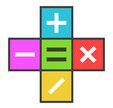
\includegraphics[scale=0.75]{front}\\

    \end{tabular}

  \end{minipage}
  &
  \begin{minipage}{8.5cm}

    \begin{center}

      {\huge \bf \titu}\\
      {\Large \bf \asig}\\ \ \\

      \convo

    \end{center}

  \end{minipage}\\ & \\ & \\  & \\

\end{tabular}

\noindent
{\Large\bf Operaciones básicas}

Todas las representaciones que se muestran a continuación se hacen
empleando las siguientes medidas:

\begin{center}
  \begin{tabular}{ll}
    \texttt{zeroheight}   & \convertto{cm}{\the\zeroheight}\ cm \\
    \texttt{zerowidth}    & \convertto{cm}{\the\zerowidth}\ cm \\
  \end{tabular}
\end{center}

\noindent
que son el alto y ancho del {\huge 0} (tamaño \texttt{$\backslash$huge}), y que
representan genéricamente el alto y ancho de cualquier carácter; y el
\texttt{baselineskip} (\convertto{cm}{\the\baselineskip}\ cm), que representa el
espacio natural entre líneas. Las dos primeras medidas mostradas arriba deben
definirse en el preámbulo del documento \LaTeX\ (por ejemplo, con un fichero
\texttt{.sty} que se incluya automáticamente en el fichero).

Hay dos tipos de operaciones diferentes: \textit{type 0} y \textit{type 1}. En
el primer caso, la caja de respuesta es el resultado de la operación, mientras
que en el segundo, el estudiante debe determinar el valor de algún operando que
produce el resultado mostrado. Además, las operaciones básicas pueden involucrar
un número cualquiera de operandos, salvo en el caso de las divisiones que nada
más que pueden ser dos. Por último, es posible definir tamto el número de
dígitos de los operandos como del resultado.

Las operaciones básicas se caracterizan con los siguientes parámetros:

\begin{itemize}

  \item Tipo de operación: \textit{type 0}

  \item Número de operandos: 2

  \item Número de dígitos de los operandos: 1

  \item Número de dígitos del resultado: 1

\end{itemize}

El esquema general se muestra a continuación:

\noindent\begin{minipage}{0.20\linewidth}
  \begin{center}
    \begin{tikzpicture}

      % --- Coordinates -----------------------------------------------------

      % Lower-left corner of the bounding box
      \coordinate (bottom) at (0,0);
      \fill [blue] (bottom) circle (1pt);

      % the result is located leaving some room to the let so that operations
      % can be drawn next to others withouth colliding. For this, the result
      % is x-shifted 1 plus half the number of digits of the result. It is
      % also always y-shifted 1.5 the baselineskip plus half the height of a
      % digit
      \coordinate (answer) at ($(bottom) + (3.0\zerowidth, 0.5\zeroheight+1.0\baselineskip)$);
      \fill [red] (answer) circle (2pt);

      % --- Split line ------------------------------------------------------

      % Next, a line splitting the operands and result is shown
      \coordinate (split1) at ($(answer) + (-2.25\zerowidth, 1.5\baselineskip)$);
      \fill [teal] (split1) circle (1pt);

      \coordinate (split2) at ($(answer) + (+1.5\zerowidth, 1.5\baselineskip)$);
      \fill [teal] (split2) circle (1pt);
      \draw [thick] (split1) -- (split2);

      % --- Operands --------------------------------------------------------

      % next, all operands are shown, as this is a type 0, they are not within
      % a box
      \coordinate (op1) at ($(answer) + (0.0, 3.0\baselineskip)$);
      \fill [red] (op1) circle (1pt);

      \coordinate (op2) at ($(answer) + (0.0, 1.0\zeroheight + 4.0\baselineskip)$);
      \fill [red] (op2) circle (1pt);

      % --- Operator --------------------------------------------------------

      % the operator is shown to the left of the first (lower) operand
      \coordinate (operator) at ($(op1) + (-2.25\zerowidth, 0.0)$);
      \fill [red] (operator) circle (1pt);

      \draw (operator) node {\huge +};

      % ---------------------------------------------------------------------

      % --- Bounding Box ----------------------------------------------------

      % the distance between the answer box and the end of the bounding box is
      % half the width of the bounding box. As this bounding box contains one
      % digit its width is 3.0 and hence 1.5 has to be multiplied by the
      % width of zero
      \coordinate (right) at ($(split2) + (0.75\zerowidth, 5.0\baselineskip)$);
      \fill [green] (right) circle (1pt);

      % % draw an invisible box used to properly align all sequences
      \draw [lightgray] (bottom) rectangle (right);

      % ---------------------------------------------------------------------

      % --- Basic operation--------------------------------------------------

      % result
      \draw(answer) node [rounded corners, rectangle, minimum width=3.0*\zerowidth, minimum height = \zeroheight + \baselineskip, draw] {\textcolor{lightgray}{\huge 7}};

      % operands
      \draw (op2) node {\huge 3};
      \draw(op2) node [lightgray, rounded corners, rectangle, minimum width=3.0*\zerowidth, minimum height = \zeroheight + \baselineskip, draw] {\textcolor{lightgray}{}};
      \draw (op1) node {\huge 4};
      \draw(op1) node [lightgray, rounded corners, rectangle, minimum width=3.0*\zerowidth, minimum height = \zeroheight + \baselineskip, draw] {\textcolor{lightgray}{}};

      % ---------------------------------------------------------------------

    \end{tikzpicture}
  \end{center}
\end{minipage}

La esquina inferior izquierda está en $(0, 0)$, y el punto de referencia del
resto de coordenadas es la caja de respuesta mostrada en la línea inferior,
con un punto rojo más grueso que los demás. La distancia desde la caja de
texto para la respuesta hasta la línea de resultados, y desde ella hasta el
primer operador (el que está justo encima de la línea de resultados) es
exactamente la misma, y es igual a 1,5 unidades de la distancia natural entre
líneas, $\backslash\mathtt{baselineskip}$.

Cada operando se circunscribe en una caja, de tal modo que todas las cajas
coinciden en uno de sus márgenes. El ancho de cada caja es el número de
dígitos que alberga más el ancho de dos dígitos, el que representa el espacio
que se deja a la derecha e izquierda. De la misma manera, cada caja deja por
encima y por debajo un espacio igual a la mitad de la altura de un dígito.

La posición del operador ($+, -, \times, \div$) se determina desplazando hacia
la izquierda el centro del primer operador (el que está justo encima de la
línea de resultados), la mitad de la caja más 0,75 unidades del ancho de un
dígito.

Es precisamente la posición del operador la que determina el ancho de la línea
de resultados, que se extiende desde justo debajo del centro del operador,
hasta el final de las cajas de los operandos y resultado.

Por último, la coordenada superior derecha se determina haciendo que la
diferencia desde el extremo derecho de la línea de resultados hasta ella, sea
igual a la distancia horizontal que hay desde la esquina inferior izquierda
hasta el extremo izquierdo de la línea de resultados, 0.75 unidades del ancho
de un dígito, y dejando por encima y por debajo una distancia igual a
$\backslash\mathtt{baselineskip}$.

La siguiente tabla muestra la forma de calcular las coordenadas $x$ e $y$ de
cada uno de los puntos de referencia empleados junto con una descripción de su
utilidad:

\begin{center}
  \begin{tabular}{c|p{2.0cm}|c|c|c}
    Etiqueta & Descripción & Referencia & $\delta x$ & $\delta y$ \\ \toprule
    \texttt{bottom} & Esquina inferior izquierda & -- & 0 & 0 \\ \midrule
    \texttt{answer} & Posición de la respuesta & \texttt{bottom}&  $1.5+\frac{2+\textrm{nbdigits}}{2}\backslash width$ & $0.5\backslash height+1.0\backslash lineskip$ \\  \midrule
    \texttt{op1} & Posición del primer operador, el que está justo encima de la línea de resultados & \texttt{answer} & 0 & $3.0\backslash lineskip$ \\  \midrule
    \texttt{op}$i$ & Posición del $i$-ésimo operador & \texttt{answer} & 0 & $3.0\backslash lineskip + (i-1) (\backslash height + \backslash lineskip)$ \\  \midrule
    \texttt{operator} & Posición del operador: $+, -, \times, \div$ & \texttt{op1} & $-\left(0.75+\frac{2+\textrm{nbdigits}}{2}\right)\backslash width$ & 0 \\  \midrule
    \texttt{split1} & Extremo izquierdo de la línea de resultaods & \texttt{answer} & $-\left(0.75+\frac{2+\textrm{nbdigits}}{2}\right)\backslash width$ & $1.5\backslash lineskip$ \\  \midrule
    \texttt{split2} & Extremo derecho de la línea de resultados & \texttt{answer} & $\left(\frac{2+\textrm{nbdigits}}{2}\right)\backslash width$ & $1.5\backslash lineskip$ \\ \midrule
    \texttt{right} & Extremo superior derecho & \texttt{split2} & $0.75\backslash width$ & $(1 + 2\times \mathrm{nbops})\backslash lineskip$ \\ \bottomrule
  \end{tabular}
\end{center}

\noindent
donde los valores del ancho y alto de un carácter o de una línea se han
abreviado por comodidad; \textit{nbdigits} representa el número máximo de
dígitos usados por todos los operados o el resultado; y \textit{nbops} es el
número de operandos.

\end{document}

%%% Local Variables:
%%% mode: latex
%%% TeX-master: t
%%% fill-column:80
%%% End:
